\documentclass{article}
\usepackage{eecstex}
\usepackage{pgfplots}
\usepackage{physics}

\DeclareMathOperator{\rect}{rect}

\title{Homework 01}
\author{Bryan Ngo}
\date{2022-01-19}

\begin{document}

\maketitle

\setcounter{section}{1}

\section{}

\subsection{}

\begin{theorem}
    The system \(L\) is not time invariant.
\end{theorem}
\begin{proof}
    We can represent a time-delayed signal as a linear combination of the other 3 signals.
    We can represent the 3 input signals in a matrix
    \begin{equation}
        \bm{X} =
        \begin{bmatrix}
           -2 & -2 & 0 \\
           1 & 1 & 1 \\
           -2 & 0 & 1 
        \end{bmatrix}
    \end{equation}
    Then, we can find the linear combination necessary to create a time delayed signal (for example, \(x_2[n - 1]\)) by solving the system of equations
    \begin{equation}
        \bm{Xa} =
        \begin{bmatrix}
            0 \\
            -2 \\
            1
        \end{bmatrix}
    \end{equation}
    where we get \(\bm{a} = \begin{bmatrix}
        -\frac{3}{2} & \frac{3}{2} & -2
    \end{bmatrix}^\top\).
    Thus, we have
    \begin{equation}
        x_2[n - 1] = -\frac{3}{2} x_1[n] + \frac{3}{2} x_2[n] - 2x_3[n]
    \end{equation}
    Calculating \(-\frac{3}{2} y_1[n] + \frac{3}{2} y_2[n] - 2y_3[n]\),
    we get the following plot:
    \begin{center}
        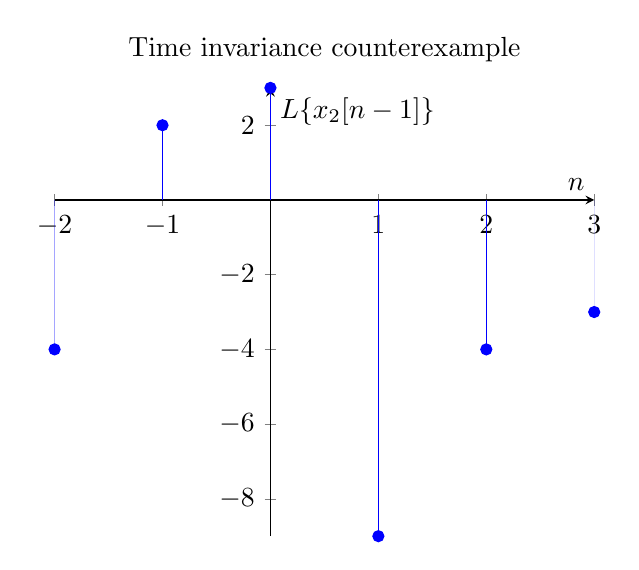
\begin{tikzpicture}
            \begin{axis}[
                xlabel=\(n\), ylabel={\(L\{x_2[n - 1]\}\)},
                title={Time invariance counterexample},
                axis lines=middle
            ]
            \addplot[
                ycomb,
                color=blue,
                mark=*
            ]
            coordinates {
                (-2, -4)
                (-1, 2)
                (0, 3)
                (1, -9)
                (2, -4)
                (3, -3)
            };
            \end{axis}
        \end{tikzpicture}
        \begin{tikzpicture}
            \begin{axis}[
                xlabel=\(n\), ylabel={\(y_2[n - 1]\)},
                title={Expected output signal},
                axis lines=middle
            ]
            \addplot[
                ycomb,
                color=blue,
                mark=*
            ]
            coordinates {
                (0, -1)
                (1, 1)
                (2, -3)
                (3, -0)
                (4, -1)
            };
            \end{axis}
        \end{tikzpicture}
    \end{center}
    So the system is \emph{not} time-invariant.
\end{proof}

\subsection{}

We can represent the delta function as
\begin{equation}
    \delta[n] = \frac{1}{2} (x_1[n] - x_2[n] + 2x_3[n])
\end{equation}
Using the properties of linear systems, we can find the impulse response
\begin{equation}
    h[n] = \frac{1}{2} (y_1[n] - y_2[n] + 2y_3[n])
\end{equation}
which gives us the following plot:
\begin{center}
    \begin{tikzpicture}
        \begin{axis}[
            xlabel=\(n\), ylabel={\(L\{\delta[n]\}\)},
            title={Impulse response},
            axis lines=middle
        ]
        \addplot[
            ycomb,
            color=blue,
            mark=*
        ]
        coordinates {
            (-2, 2)
            (-1, 1)
            (0, -2)
            (1, 3)
            (2, 2)
            (3, 1)
        };
        \end{axis}
    \end{tikzpicture}
\end{center}

\newpage
\section{}

\begin{align}
    y[n] - ay[n - 1] &= x[n] \\
    y[0] &= 1
\end{align}

\subsection{}

By counterexample, consider \(x[n] = \delta[n]\) and \(n = 1\),
\begin{equation}
    y[1] = a
\end{equation}
Then, consider \(x[n - 1] = \delta[n - 1]\) and \(n = 1\),
\begin{equation}
    y[1] - a y[0] = \delta[0] \implies y[1] = 1 + a
\end{equation}
whereas \(y[n - 1] = y[0] = 1\) by the initial condition.
So the system is not time-invariant.

\subsection{}

Given the initial condition \(y[0] = 1\), scaling the input does not change this fact, so the system \emph{cannot} be linear.

\subsection{}

The system is still not time-invariant due to the same counterexample as above.
The system is now linear as we can see because we no longer have an affine transformation at \(y[0]\).

\newpage
\section{}

\begin{equation}
    y[n] = h[n] \ast (\cos[\omega_0 n] x[n]) = \sum_{k \geqslant 0} \frac{1}{1 + k} \cos[\omega_0 (n - k)] x[n - k]
\end{equation}

\subsection{}
Proving linearity, suppose we are given the system responses \(x_1[n] \iff y_1[n]\) and \(x_2[n] \iff y_2[n]\),
\begin{align}
    T\{ax_1[n] + bx_2[n]\} &= h[n] \ast (\cosine[\omega_0 n] (ax_1[n] + bx_2[n])) \\
    &= h[n] \ast (\cos[\omega_0 n] ax_1[n] + \cos[\omega_0 n] bx_2[n]) \\
    &= a (h[n] \ast \cos[\omega_0 n] x_1[n]) + b (h[n] \ast \cos[\omega_0 n] x_2[n]) \\
    &= ay_1[n] + by_2[n]
\end{align}
For time invariance,
\begin{align}
    T\{x[n - n_0]\} &= h[n] \ast (\cosine[\omega_0 n] x[n - n_0]) \\
    y[n - n_0] &= h[n - n_0] \ast (\cosine[\omega_0 (n - n_0)] x[n - n_0])
\end{align}
The two are clearly not the same, so our system is not time invariant and thus not LTI.

\subsection{}

We can bound the cosine function with 1.
Similar to Example 2.18 in Oppenheim \& Schafer, if \(|x[n]| < B_x\),
\begin{equation}
    |y[n]| = \sum_{k \geqslant 0} \frac{1}{1 + k} B_x = B_x \sum_{k \geqslant 1} \frac{1}{k}
\end{equation}
which is a divergent harmonic series.

\subsection{}

The system is causal since the \(y[n]\) consists of a memoryless multiplication by a cosine function and convolution with a causal LTI system, which makes the system overall causal.

\newpage
\section{}

\subsection{}

We can model the frequency response as
\begin{equation}
    H(e^{j \omega}) =
    \begin{cases}
        1 & |\omega| < \frac{\pi}{2} \\
        0 & \text{elsewhere}
    \end{cases}
\end{equation}
Finding the inverse Fourier transform,
\begin{align}
    h[n] &= \frac{1}{2\pi} \int_{-\pi}^\pi H(e^{j \omega}) e^{j \omega n} \, d\omega \\
    &= \frac{1}{2\pi} \int_{-\frac{\pi}{2}}^{\frac{\pi}{2}} e^{j \omega n} \, d\omega = \frac{1}{2\pi} \eval{\frac{e^{j \omega n}}{jn}}_{-\frac{\pi}{2}}^{\frac{\pi}{2}} \\
    &= \frac{1}{2\pi j n} \left(e^{j \frac{\pi}{2} n} - e^{-j \frac{\pi}{2} n}\right) = \frac{\sin\left[\frac{\pi}{2} n\right]}{\pi n}
\end{align}

\subsection{}

The system is not causal, since \(h[-1] = \frac{1}{\pi} \neq 0\).

\subsection{}

This is a specific case of Example 2.18 in Oppenheim \& Schafer.
Each term of the absolute sum of the sinc function only decreases on the order of \(\frac{1}{n}\), so we can treat the sum as the harmonic series, which diverges.
Thus, the low pass filter is not BIBO stable.

\newpage
\section{}

\begin{equation}
    y[n] = \frac{1}{6} \sum_{k = 0}^5 x[n - k]
\end{equation}

\subsection{}

Using Equation 2.123 from Oppenheim \& Schafer with \(M = 5\),
\begin{align}
    H(e^{j \omega}) &= \frac{1}{6} \frac{\sin(3\omega)}{\sin\left(\frac{\omega}{2}\right)} e^{-j \frac{5}{2} \omega} \\
    |H(e^{j \omega})| &= \frac{1}{6} \left|\frac{\sin(3\omega)}{\sin\left(\frac{\omega}{2}\right)}\right| \\
    \angle H(e^{j \omega}) &= -\frac{5}{2} \omega \\
\end{align}
The zero crossings are \(\omega = \frac{k\pi}{3}\) for nonzero \(k \in \Z\), by solving for the equation \(\sin(3\omega) = 0\).
\begin{center}
    \begin{tikzpicture}
        \begin{axis}[
            xlabel=\(\omega\), ylabel={\(|H(e^{j \omega})|\)},
            title={Magnitude of Frequency Response},
            axis lines=middle,
            ymin=0, ymax=1,
            width=0.4\textwidth
        ]
        \addplot[color=blue] table[
            col sep=comma,
            x=n, y=q6a-mag
        ]{q6a-mag.csv};
        \end{axis}
    \end{tikzpicture}
    \begin{tikzpicture}
        \begin{axis}[
            xlabel=\(\omega\), ylabel={\(\angle H(e^{j \omega})\)},
            title={Phase of Frequency Response},
            axis lines=middle,
            width=0.4\textwidth
        ]
        \addplot[color=blue] table[
            col sep=comma,
            x=n, y=q6a-ang
        ]{q6a-ang.csv};
        \end{axis}
    \end{tikzpicture}
\end{center}

\subsection{}

Let \(\omega_1 = \frac{\pi}{3}\).
Then, the output \(y[n]\) is as shown:
\begin{center}
    \begin{tikzpicture}
        \begin{axis}[
            xlabel=\(n\), ylabel={\(y[n]\)},
            title={Convolution Sum},
            axis lines=middle,
            width=0.4\textwidth
        ]
        \addplot[ycomb, mark=*, color=blue] table[
            col sep=comma,
            x=n, y=q6b
        ]{q6b.csv};
        \end{axis}
    \end{tikzpicture}
\end{center}
The transient at the start of the convolution sum comes from at the beginning of the MAF, where the positive terms from the first 2 inputs of the cosine function.
The settling of the convolution sum comes from the fact that the sum of a sinusoid without a vertical shift over 1 period is 0. Since the MAF has a window of size 6, and the cosine has a period of 6 as well, once the window is filled by the cosine, it we get 0.
For any value of the convolution sum afterwards, it remains 0 due to the MAF now being saturated with a constant 1 period of the cosine, which has a sum of 0.

\newpage
\section{}

\begin{equation}
    y[n] = \mathcal{P}\{x[n - 2], x[n - 1], x[n], x[n + 1], x[n + 2]\}
\end{equation}

\subsection{}

We can transform the problem into a least-squares problem:
\begin{equation}
    \begin{bmatrix}
        x[-2] \\
        x[-1] \\
        x[0] \\
        x[1] \\
        x[2]
    \end{bmatrix}
    = 
    \begin{bmatrix}
        1 & -2 & 4 \\
        1 & -1 & 1 \\
        1 & 0 & 0 \\
        1 & 1 & 1 \\
        1 & 2 & 4
    \end{bmatrix}
    \begin{bmatrix}
        a_0 \\
        a_1 \\
        a_2
    \end{bmatrix}
\end{equation}
By the least squares formula \(\bm{\hat{a}} = (\bm{P}^\top \bm{P})^{-1} \bm{P}^\top \bm{x}\), we get that
\begin{align}
    \begin{bmatrix}
        a_0 \\
        a_1 \\
        a_2
    \end{bmatrix}
    &=
    \frac{1}{35} \begin{bmatrix}
        -3 & 12 & 17 & 12 & -3 \\
        -7 & -3.5 & 0 & 3.5 & 7 \\
        5 & -2.5 & -5 & -2.5 & 5
    \end{bmatrix}
    \begin{bmatrix}
        x[-2] \\
        x[-1] \\
        x[0] \\
        x[1] \\
        x[2]
    \end{bmatrix} \\
    \implies y[0] &= a_0 = \frac{1}{35} (-3x[-2] + 12x[-1] + 17x[0] + 12x[1] - 3x[2])
\end{align}

\subsection{}

\begin{equation}
    \begin{bmatrix}
        x[-1] \\
        x[0] \\
        x[1] \\
        x[2] \\
        x[3]
    \end{bmatrix}
    = 
    \begin{bmatrix}
        1 & -2 & 4 \\
        1 & -1 & 1 \\
        1 & 0 & 0 \\
        1 & 1 & 1 \\
        1 & 2 & 4
    \end{bmatrix}
    \begin{bmatrix}
        a_0 \\
        a_1 \\
        a_2
    \end{bmatrix}
\end{equation}
which gives us the solution
\begin{equation}
    y[1] = a_0 = \frac{1}{35} (-3x[-1] + 12x[0] + 17x[1] + 12x[2] - 3x[3])
\end{equation}

\subsection{}

The system is linear since it entirely consists of additions and scalar multiplications.
The system is time-invariant since for any shift \(n_0\), the corresponding \(x[n - n_0]\) is simply shifted and put into the solution, which is what is expected for a time-shifted output.
The system is stable since if \(x[n]\) is bounded by \(B_x\), \(y[n]\) is bounded by \(B_x\).
Since the system is LTI, the system has a frequency response.
We do not actually need to perform a regression for every \(n\), since the coefficient matrix multiplying the set of \(x[n - k]\) is constant.

\subsection{}

We can see that points further from the operating point have the largest weights, while weights further away have smaller and even negative weights.
This means that it better represents a distribution around a local region, and does not flatten out features as drastically as a standard MAF.

\end{document}
